\documentclass[a4paper, 12pt]{article} % тип документа

%%%Библиотеки
	%\usepackage[warn]{mathtext}	
	\usepackage[T2A]{fontenc}   %Кодировка
	\usepackage[utf8]{inputenc} %Кодировка исходного текста
	\usepackage[english, russian]{babel} %Локализация и переносы
	\usepackage{caption}
	\usepackage{listings}
	\usepackage{amsmath, amsfonts, amssymb, amsthm, mathtools}
	\usepackage[warn]{mathtext}
	\usepackage[mathscr]{eucal}
	\usepackage{wasysym}
	\usepackage{graphicx} %Вставка картинок правильная
	\DeclareGraphicsExtensions{.pdf,.png,.jpg}
	\graphicspath{ {images/} }
	
	\setlength{\parskip}{0.5cm}
	
	\usepackage{pgfplots}
	\usepackage{indentfirst}
	\usepackage{float}    %Плавающие картинки
	\usepackage{wrapfig}  %Обтекание фигур (таблиц, картинок и прочего)
	\usepackage{fancyhdr} %Загрузим пакет
	\usepackage{lscape}
	\usepackage{xcolor}
	\usepackage[normalem]{ulem}
	\usepackage{wasysym}
	
	\usepackage{titlesec}
	\titlelabel{\thetitle.\quad}

	\usepackage{hyperref}
	\newenvironment{comment}{}{}

%%%Конец библиотек

%%%Настройка ссылок
	\hypersetup
	{
		colorlinks = true,
		linkcolor  = blue,
		filecolor  = magenta,
		urlcolor   = blue
	}
%%%Конец настройки ссылок


%%%Настройка колонтитулы
	\pagestyle{fancy}
	\fancyhead{}
	\fancyhead[L]{2.4.1}
	\fancyhead[R]{Старченко Иван, группа Б01-005}
	\fancyfoot[C]{\thepage}
%%%конец настройки колонтитулы

\begin{document}

%\maketitle
%\thispagestyle{empty}

%\newpage
\setcounter{page}{1}

\begin{center}
  \LARGE{Лабораторная работа 2.4.1}\\[0.2cm]
  \LARGE{Определения теплоты испарения жидкости.}\\[0.2cm]
  \large{10 Марта 2021 г.}\\[0.2cm]
  \large{Старченко Иван Александрович}\\[0.2cm]
\end{center}


						%%%%Начало документа%%%%

\textbf{Цель работы:} измерение давления насыщенного пара жидкости при разной температуре; вычисление по полученным данным теплоты испарения с помощью уравнения Клапейрона–Клаузиуса.\\

\textbf{Используемое оборудование:} термостат; герметический сосуд, заполненный исследуемой жидкостью; отсчетный микроскоп.

\section{Теоретическое введение}

Теплоту парообразования жидкостей можно измерить непосредственно при помощи калориметра. Такой метод, однако, не позволяет получить точных результатов из-за неконтролируемых потерь тепла, которые трудно сделать малыми. В настоящей работе для определения теплоты испарения применен
косвенный метод, основанный на формуле Клапейрона–Клаузиуса: 

\begin{equation}
	\frac{dP}
{dT} = \frac{L}{T(V_2 - V_1)}
\end{equation}

Здесь $P$ — давление насыщенного пара жидкости при температуре $T$, $T$ — абсолютная температура жидкости и пара, $L$ — теплота испарения жидкости, $V2$ — объем пара, $V_1$ — объем жидкости. Найдя из опыта $\frac{dP}{dT},\; T,\; V_2$ и $V_1$, можно определить $L$ путем расчета. Величины $L, \;V_2$ и $V_1$ в формуле $(1)$ должны относиться к одному и тому же количеству вещества; мы будем относить их к одному молю.
В нашем приборе измерения производятся при давлениях ниже атмосферного. В этом случае задача существенно упрощается.

С помощью уравнения Ван-дер-Ваальса можно получить зависимость $P(T)$, с помощью которой определить искомую величину:

\begin{equation}
	\left(P+\frac{a}{V^2}\right)(V-b) = RT
\end{equation}

В таблице ниже приведены все значения параметров различных жидкостей уранения Ван-дер-Ваальса в условиях данного опыта.

\begin{figure}[h]
	\center{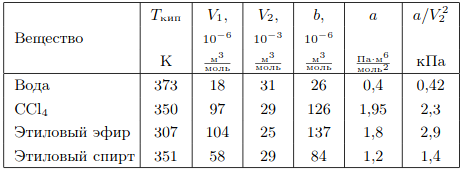
\includegraphics[scale = 1]{data_standart}}
\end{figure}

Откуда видно, что $\frac{V_1}{V_2} < 0,005$, a $\frac{a}{PV^2}<0,03$, ошибка метода измерений равна $4\%$, тогда записав уравнение Клапейрона-Менделеева для насыщенного пара, получим:
$V=\frac{RT}{P}\;.$
Пренебрегая $V_1$ (который не превосходит $0,5\%$ от $V_2$), запишем:

\begin{equation}
	L=\frac{RT^2}{P} \frac{dP}{dT} = -R\frac{d(lnP)}{d(1/T)}
\end{equation}

Эта формула является окончательной.

\section{Эксперементальная установка}

Схема установки изображена на рисунке $1$. Наполненный водой резервуар $1$ играет роль термостата. Нагревание термостата производится спиралью $2$, подогреваемой электрическим током. Для охлаждения воды в термостате через змеевик $3$ пропускается водопроводная вода. Вода в термостате перемешивается воздухом,
поступающим через трубку $4$. Температура воды измеряется термометром $5$. В термостат погружен запаянный прибор $6$ с исследуемой жидкостью. Над ней находится насыщенный пар (перед заполнением прибора воздух из него был откачан).
Давление насыщенного пара определяется по ртутному манометру,соединенному с исследуемым объемом. Отсчет показаний манометра производится при помощи микроскопа.

\begin{figure}[h]
	\center{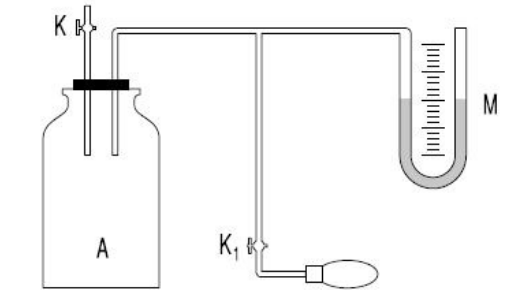
\includegraphics[scale = 1]{ustan}}
	\caption{Схема установки для определения теплоты испарения}
\end{figure}

\section{Снятие данных}

Измерим разность уровней в ртутном $U$-образном манометре с помощью микроскопа и температуру по термометру. $H$ - высота высокого колена, $h$ - низкого. При этом будем настраивать микроскоп так, чтобы каждый раз основание мениска было у метки прибора (в дальнейшем считаем, что высота мениска не меняется, не смотря на то что поверхностное натяжение ртути на самом деле зависит от температуры и высота немного должна меняться). Результаты представлены в таблицах $1$ и $2$. Под $P_0$ подразумевается давление $1$ мм рт.ст.

Приведём формулы для рассчётов погрешностей.
Поскольку давление напрямую зависит от разности уровней ртути (пренебрегаем давлением насыщенных паров ртути, так как при комнатной температуре оно приблизительно равно $0,24$ Па, а так же изменением уровня столба воды, так как он слишком мал), то для погрешности давления $P$ воспользуемся следующей формулой: 

\begin{equation}
	\sigma_P = P_{\text{aтм}} \cdot \frac{\sigma_{H-h}}{H_0}
\end{equation}

где под $H_0$ подразумевается $760$ мм, а под $P_{\text{атм}} = 101325 \; \text{Па}$ - нормальное атмосферное давленине. В качестве $\sigma_{H-h}$ будем брать $2$ мм, поскольку точность измерения каждого из уровня $0,1$ мм, а так же мы будем учитывать, что $U$-образный манометр в нашей установке был не вертикален, а немного наклонён.

\begin{equation}
	\sigma_{\ln{\frac{P}{P_0}}} = \frac{\sigma_P}{P}
\end{equation}

Погрешность определения температуры возьмём учитывая точность прибора и тот факт, что во время измерений уровней температура могла немного изменяться: $\sigma_{T} = 0,2 \; K$.

Соответсвенно

\begin{equation}
	\sigma_{\frac{1}{T}} = \frac{\sigma_T}{T^2}
\end{equation}

Снимем все точки данных, проведя сам эксперимент (см. таблицы, приведены в конце).

\section{Аппроксимация полученных данных}

Как было сказано в теоретическом введении, согласно формуле $(3)$, график зависимости $ln(P)\left( \frac{1}{T}\right)$ -- убывающая прямая. Учитывая, что известны погрешности $\sigma_{ln(P)} \gg \sigma_{\frac{1}{T}}$, определим характеристики прямой графика с помощью МНК в программе MATLAB по следующим формулам:

\begin{equation}
	L_1 = \frac{\langle ln(P) \rangle \cdot \langle \frac{1}{T} \rangle - \langle \frac{ln(P)}{T} \rangle}{\langle \frac{1}{T^2} \rangle  - \left( \langle \frac{1}{T} \rangle  \right)^2}
\end{equation}

\begin{equation}
	L_2 = \frac{R\cdot \langle T \rangle^2}{\langle P \rangle}\cdot\frac{\langle P \rangle \cdot \langle T \rangle - \langle P\cdot T \rangle}{\langle T^2 \rangle  -  \langle T \rangle^2}
\end{equation}


\begin{equation}
	\delta_{L} = \sqrt{\frac{1}{n(n-1)}\sum_{i=1}^n(L_i - \langle L\rangle)^2}
\end{equation}

По этим формулам получим следующие значения при нагревании:

\begin{equation}
	L_{\text{н}1} = 2,69 \cdot 10^6 \; \frac{\text{Дж}}{\text{К}}, \Delta L_{\text{н}1} = 9,86 \cdot 10^4 \; \frac{\text{Дж}}{\text{К}}\;
\end{equation}

\begin{equation}
	L_{\text{н}2} = 2,81 \cdot 10^6 \; \frac{\text{Дж}}{\text{К}}, \Delta L_{\text{н}2} = 11,73 \cdot 10^4 \; \frac{\text{Дж}}{\text{К}}\;
\end{equation}

\begin{equation}
	L_{\text{охл}1} = 2,83 \cdot 10^6 \; \frac{\text{Дж}}{\text{К}}, \Delta L_{\text{охл}1} = 9,65 \cdot 10^4 \; \frac{\text{Дж}}{\text{К}}\; 
\end{equation}

\begin{equation}
	L_{\text{охл}2} = 3,01 \cdot 10^6 \; \frac{\text{Дж}}{\text{К}}, \Delta L_{\text{охл}2} = 12,01 \cdot 10^4 \; \frac{\text{Дж}}{\text{К}}\; 
\end{equation}

Заметим, что значение удельной теплоты парообразования воды при нагревании для $ln(p)(\frac{1}{T})$ больше всего приближенна к табличным данным ($L = 2,44 \cdot 10^6 \; \frac{\text{Дж}}{\text{К}}$)

Теперь нужно учесть погрешности, вызванные методическими приближениями. 

Первое, что нужно учесть -- давление насыщенного пара ртути, которым мы пренебрегли при расчёте погрешностей ввиду его малости по сравнению с атмосферным давлением:

\begin{equation}
	\frac{\Delta L_P  }{L} = \frac{P_s}{P} = \frac{0,26}{3 \cdot 10^3} = 8,667 \cdot 10^{-5}
\end{equation}

Эта формула следует напрямую из уравнения Клапейрона-Клаузиуса.

Теперь посчитаем относительную погрешность:

\begin{equation}
	\epsilon_{\text{н1}} = \frac{\Delta L_{\text{н1}}}{L_{\text{н1}}} = 0,0367
\end{equation}

\begin{equation}
	\epsilon_{\text{охл1}} = \frac{\Delta L_{\text{охл1}}}{L_{\text{охл1}}} = 0,0417
\end{equation}

\begin{equation}
	\epsilon_{\text{н2}} = \frac{\Delta L_{\text{н2}}}{L_{\text{н2}}} = 0,034
\end{equation}

\begin{equation}
	\epsilon_{\text{охл2}} = \frac{\Delta L_{\text{охл2}}}{L_{\text{охл2}}} = 0,0420
\end{equation}


Стоить отметить, что погрешности вышли заниженными, так как следует учитывать также следующие факторы, которые измерить тяжело: температура термометра в точности не совпадает с температурой пара из-за неравномерности распределения температуры в термостате, из-за капиллярных эффектов давление насыщенного пара должно быть больше, чем просто разность высот в трубках.

Всё же можно видеть, что полученные значения хорошо соответствуют ранее описанной теории. Для убедительности построим графики $P(T)$ и $ln(P)\left( \frac{1}{T}\right)$ и проведем сглаживающие прямые по методу МНК с помощью программы MATLAB.


\section{Заключение}

В работе изучалась зависимость давления насыщенного пара воды от температуры. По полученным данным были найдены коэффициенты удельного испарения воды при нагревании и охлаждении жидкости и были вычислены все возможные погрешности полученных величин.


Полученное в результате работы из зависимости $ln(P)\left(\frac{1}{T}\right)$ при нагревании, $L$ получилось наиболее приближенное к табличному значнию, но всё-таки  получилось не очень точное, на это повляли факторы описанные выше. Различие с табличными:
\begin{equation}
	\eta = \frac{L_\text{н} - L_\text{табл}}{L_\text{табл}}\cdot 100\% = 10,24 \% 
\end{equation}

\section{Список используемой литературы}

$\bullet$ Гладун А. Д. Лабораторный практикум по общей физике. Термодинамика и молекулярная физика\\

$\bullet$ \href{https://mipt.ru/education/chair/physics/S_II/lab/}{Описание лабораторных работ на кафедре общей физики МФТИ}

\newpage

\section{Графики}

\begin{figure}[h]
	\center{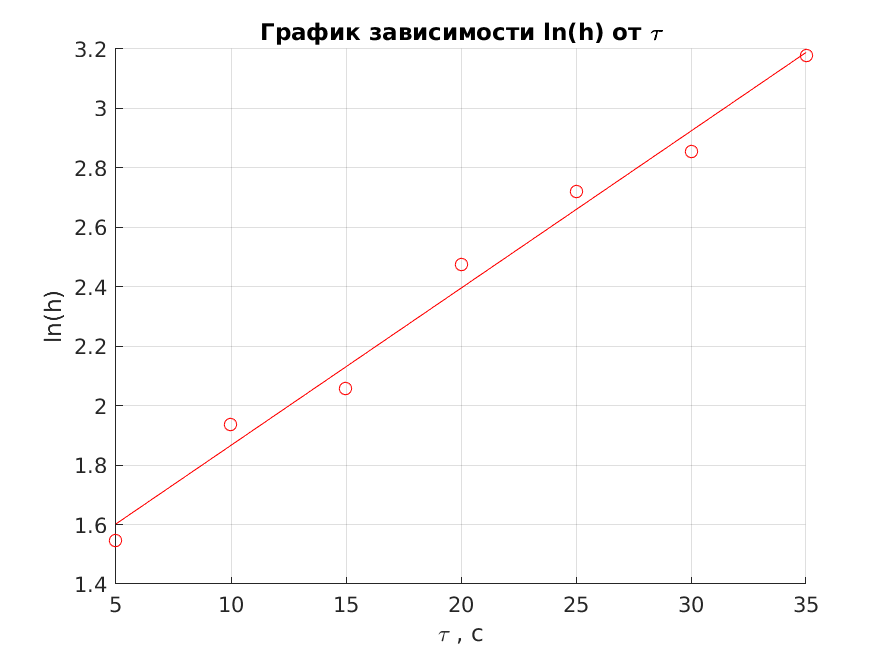
\includegraphics[scale = 0.68]{graph_1}}
\end{figure}

\begin{figure}[h]
	\center{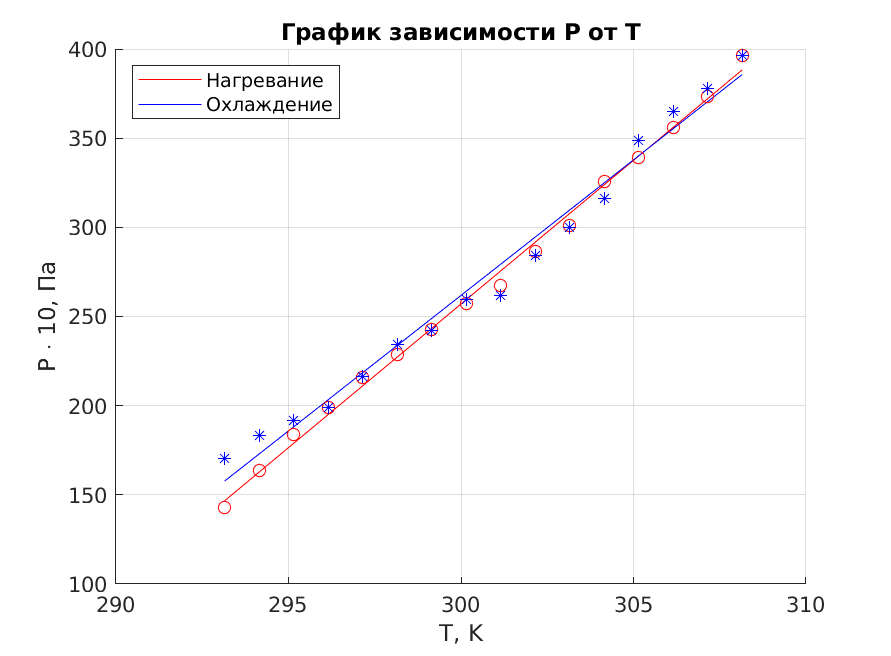
\includegraphics[scale = 0.68]{graph_2}}
\end{figure}

\begin{center}
\begin{table}[h]
		\caption{При нагреве}
\begin{tabular}{|c|c|c|c|c|c|c|c|c|c|c|} \hline
$N$ & $T, C$ & $T, K$ & $h(\text{б}), \text{мм}$ & $h(\text{м}), \text{мм}$ & $\Delta h, \text{мм}$ & $P, Па$ & $Ln(P)$ & $1/T\cdot10^{-3}, 1/K$ \\ \hline
 1 & 20 & 293.15 &  90.60 & 76.00 & 14.60 & 142.97 & 4.96 & 3.41  \\ \hline
 2 & 21 & 294.15 &  91.60 & 74.90 & 16.70 & 163.53 & 5.10 & 3.40  \\ \hline 
 3 & 22 & 295.15 &  92.25 & 73.45 & 18.80 & 184.10 & 5.22 & 3.39  \\ \hline
 4 & 23 & 296.15 &  92.65 & 72.35 & 20.30 & 198.78 & 5.29 & 3.38  \\ \hline
 5 & 24 & 297.15 &  93.50 & 71.45 & 22.05 & 215.92 & 5.37 & 3.37  \\ \hline
 6 & 25 & 298.15 &  94.35 & 71.00 & 23.35 & 228.65 & 5.43 & 3.35  \\ \hline
 7 & 26 & 299.15 &  95.25 & 70.45 & 24.80 & 242.85 & 5.49 & 3.34  \\ \hline
 8 & 27 & 300.15 &  95.65 & 69.35 & 26.30 & 257.54 & 5.55 & 3.33  \\ \hline
 9 & 28 & 301.15 &  96.55 & 69.25 & 27.30 & 267.33 & 5.59 & 3.32  \\ \hline
10 & 29 & 302.15 &  96.90 & 67.65 & 29.25 & 286.43 & 5.66 & 3.31  \\ \hline
11 & 30 & 303.15 &  98.25 & 67.50 & 30.75 & 301.11 & 5.71 & 3.30  \\ \hline
12 & 31 & 304.15 &  99.00 & 64.40 & 34.60 & 338.82 & 5.83 & 3.29  \\ \hline
13 & 32 & 305.15 &  99.45 & 65.65 & 33.80 & 330.98 & 5.80 & 3.28  \\ \hline
14 & 33 & 306.15 & 100.95 & 64.60 & 36.35 & 355.95 & 5.87 & 3.27  \\ \hline
15 & 34 & 307.15 & 101.95 & 63.85 & 38.10 & 373.09 & 5.92 & 3.26  \\ \hline
16 & 35 & 308.15 & 103.85 & 63.35 & 40.50 & 396.59 & 5.98 & 3.25  \\ \hline
\end{tabular}\\\\
	\caption{При охлаждении}
\begin{tabular}{|c|c|c|c|c|c|c|c|c|c|c|} \hline
$N$ & $T, C$ & $T, K$ & $h(\text{б}), \text{мм}$ & $h(\text{м}), \text{мм}$ & $\Delta h, \text{мм}$ & $P, Па$ & $Ln(P)$ & $1/T\cdot10^{-3}, 1/K$ \\ \hline
 1 & 35 & 308.15 & 103.85 & 63.35 & 40.50 & 396.59 & 5.98 & 3.25  \\ \hline
 2 & 34 & 307.15 & 102.35 & 63.75 & 38.60 & 377.98 & 5.93 & 3.26  \\ \hline
 3 & 33 & 306.15 & 101.80 & 64.55 & 37.25 & 364.76 & 5.90 & 3.27  \\ \hline
 4 & 32 & 305.15 & 101.25 & 65.65 & 35.60 & 348.61 & 5.85 & 3.28  \\ \hline
 5 & 31 & 304.15 & 100.15 & 66.65 & 32.30 & 316.29 & 5.76 & 3.29  \\ \hline
 6 & 30 & 303.15 &  99.25 & 67.85 & 30.65 & 300.14 & 5.70 & 3.30  \\ \hline
 7 & 29 & 302.15 &  98.00 & 68.60 & 29.05 & 284.47 & 5.65 & 3.31  \\ \hline
 8 & 28 & 301.15 &  96.75 & 68.95 & 26.75 & 261.95 & 5.57 & 3.32  \\ \hline
 9 & 27 & 300.15 &  96.50 & 70.00 & 26.50 & 259.50 & 5.56 & 3.33  \\ \hline
10 & 26 & 299.15 &  95.75 & 71.00 & 24.75 & 242.36 & 5.49 & 3.34  \\ \hline
11 & 25 & 298.15 &  94.60 & 70.65 & 23.95 & 234.53 & 5.46 & 3.35  \\ \hline
12 & 24 & 297.15 &  93.85 & 71.75 & 22.10 & 216.41 & 5.38 & 3.37  \\ \hline
13 & 23 & 296.15 &  92.95 & 72.65 & 20.30 & 198.78 & 5.29 & 3.38  \\ \hline
14 & 22 & 295.15 &  92.40 & 72.85 & 19.55 & 191.44 & 5.25 & 3.39  \\ \hline
15 & 21 & 294.15 &  92.35 & 73.65 & 18.70 & 183.12 & 5.21 & 3.40  \\ \hline
16 & 20 & 293.15 &  92.15 & 74.73 & 17.42 & 170.58 & 5.14 & 3.41  \\ \hline
\end{tabular}
\end{table}
\end{center}


\end{document}